\section{Related Work}\label{sec:relatedWorks}

\todo{Revise and refine}
Some of the variability points can be handled differently. The initial assumption of our research was that the collection of the variants had to be done explicitly, which implied that run time variability and internal binding was required~\cite{JillesVanGurp2001}. %\todo{(Svahnberg, van Gurp \& Bosch, 2005)}. 
While we choose not to follow this path for the rest of our study, mainly due to the feedback we got from the company's stakeholders, some of the variation points can still be handled at run time. The main reason for this argument is that this was the case in the old system. 


\subsection{Trade-off Analysis of Variability Realization Mechanisms}

We have discussed in a previous section about the main realization mechanisms for variability, found in the generic literature. In this section we present the strengths and weaknesses for each of these mechanisms.

\subsubsection{Generators}
According to an experience report for variability management in the field of avionics~\cite{Wolfl2015} generators can follow an asset-based development dividing the work to domain and application engineering and generating source code. This approach is more suitable when a large number of variation points is expected. This is also supported by~\cite{Bachmann2001}. % (Bachmann \& Bass 2001 p7) 
The benefit is that the quality of code increases and only the generator is needed to be maintained and evolved to support new variability points and also enhances the understandability of the system. The weakness of this technique is the upfront investment that is required since generators imply the development of meta models, domain specific languages and transformation rules, as mentioned in~\cite{Wolfl2015} and~\cite{Bachmann2001}. %(Bachmann \& Bass 2001 p7).

\subsubsection{Configuration management systems}

Additionally, this approach is efficient when dealing with alternative implementations and it is easier to maintain. However, it is difficult to manage optional features and, like the generator, it requires upfront investment although probably not as expensive as building a generator~\cite{Bachmann2001}. This approach implies that the company maintains customer specific modules from its side. An alternative to this approach is simply making use of version control systems to keep track of the different implementations of a module. %(SEI 2000 p53)

\subsubsection{Self-Adaptive systems}

According to~\cite{vandenHeuvel2007}, %(Van den Heuvel, Weigand, Hiel. 2007), 
this approach is more suitable for the automation of solving interoperability conflicts through the use of learning mechanisms rather than handling variability issues. Strong emphasis is placed on addressing performance issues. The effort required to define the algorithm which chooses the best of the available options require some significant effort. 

\subsubsection{Code level approaches } 

Code level, or lower level approaches, require less effort to implement but due the manual effort which is required, they might not be suitable for a large number of requirements~\cite{Wolfl2015}. 
As mentioned in previous chapter, there are many ways to make use of code level techniques. Object oriented mechanisms include techniques such as inheritance, extensions and polymorphism~\cite{Gacek2001}. %(Anastasopoulos \& Gacek. 2001) (Lee, Hwang 2014). 
Design patterns where the benefits and drawbacks are known beforehand~\cite{Gamma1995} can influence our decision. Furthermore, code level techniques can provide hybrid approaches. In the variability realization mechanisms of the taxonomy in~\cite{JillesVanGurp2001} % (Svahnberg, Gurp, Bosch 2005) 
some of the approaches make use of combination of design patterns, mainly to handle run time variability. Additionally, for build time binding, there are approaches which make use of configuration management tools and architecture reorganization.

\subsubsection{Summary } 
In Figure~\ref{fig:strenghtsWeaknesses} we summarize the main available methods with their strengths and weaknesses. 


\iffalse
\begin{table}[H]
\centering 


%\caption{Summary}
\label{my-label}
\begin{tabular}{l l l l  }
\hline\hline 
Method & Description & Strengths & Weaknesses \\ 
\hline 
 Generators  & Generates customer & Powerful tool for large & Upfront investment \\ 
             & specific artifacts based  & number of use cases &   \\ 
             & on a given input &   & \\
[1ex]
\hline 

Configuration & Produces  & Efficient when dealing with  & Requires\\ 
Management    & customer specific & alternative Implementations & maintenance of  \\ 
Systems       & modules. & Easier to maintain. & customer specific   \\ 
              &   &   & modules \\
[1ex]
\hline 

Self-adaptive & Selection from a & Automatically solves protocol & More suitable for \\
systems       & repository of scripts, & mismatches. Strong emphasis & networked systems.\\
& dynamically, based on & on performance. & Requires sophisticated \\
& the state of the system. &   &   algorithms\\
[1ex]
\hline

Code level & Software engineering & Easier to introduce. & Not suitable for too  \\
methods    & and product line & Effective when the number of & many use cases \\
           & engineering patterns. & use cases is not large. &   \\
[1ex]
\hline
\end{tabular}
\caption{Summary of main methods}
\end{table}


\fi


\begin{figure*}[h]
\centering
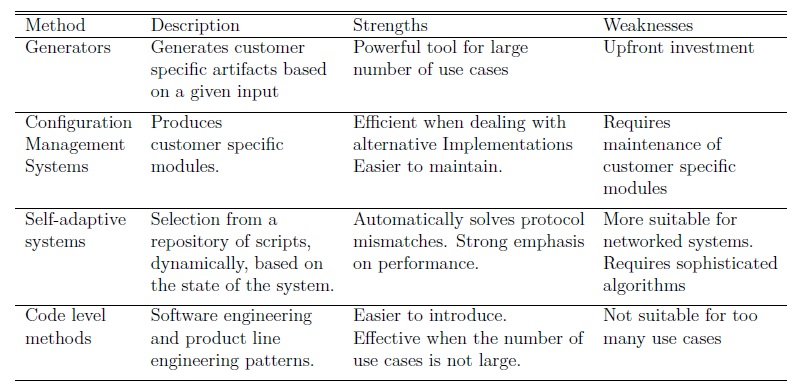
\includegraphics[width=.8\textwidth]{figure/figure14.jpg}
\caption{Summary of strengths and weaknesses of the main methods}
\label{fig:strenghtsWeaknesses}
\end{figure*}




A generator would require too significant upfront investment. Additionally, there are currently not enough identified use cases. Therefore, the return of investment can not be easily estimated. 

To make use of Configuration Management Tools include a cost of their purchase. Alternatively, the existing version control systems of the company could suffice. The problem of this approach is that maintaining a history of changes of each customer specific components and configuration still requires effort~\cite{Bachmann2001}.  %(Bachmann \& Bass 2001 p7). 
This technique could be a viable approach if there were more concrete use cases and there was an urgent need to maintain all these different components from the side of Jeppesen.

Self-adaptive systems is a more viable approach for networked systems. However, maintaining a knowledge-base where the appropriate script to handle a certain situation could be proved viable, especially for run time binding.

Code level techniques appear to be more suitable in the case of the investigated interface. The main argument to support this decision is that the number of possible customer specific requirements is not expected to be too high. There is a significant number of different techniques. %We choose to follow the general grouping discussed in (V�lter, 2009), which is the removal, injection and parametrization as we discussed in 3.7.4.2. 
For adopting a more concrete realization mechanism, we choose to follow the taxonomy of~\cite{JillesVanGurp2001}. % (Svahnberg, Gurp, Bosch 2005). 
In figure 5.4 we borrow their summary. The indicators which we discussed previously can help us choose among those methods. 



%\begin{figure*}[h]
%\centering
%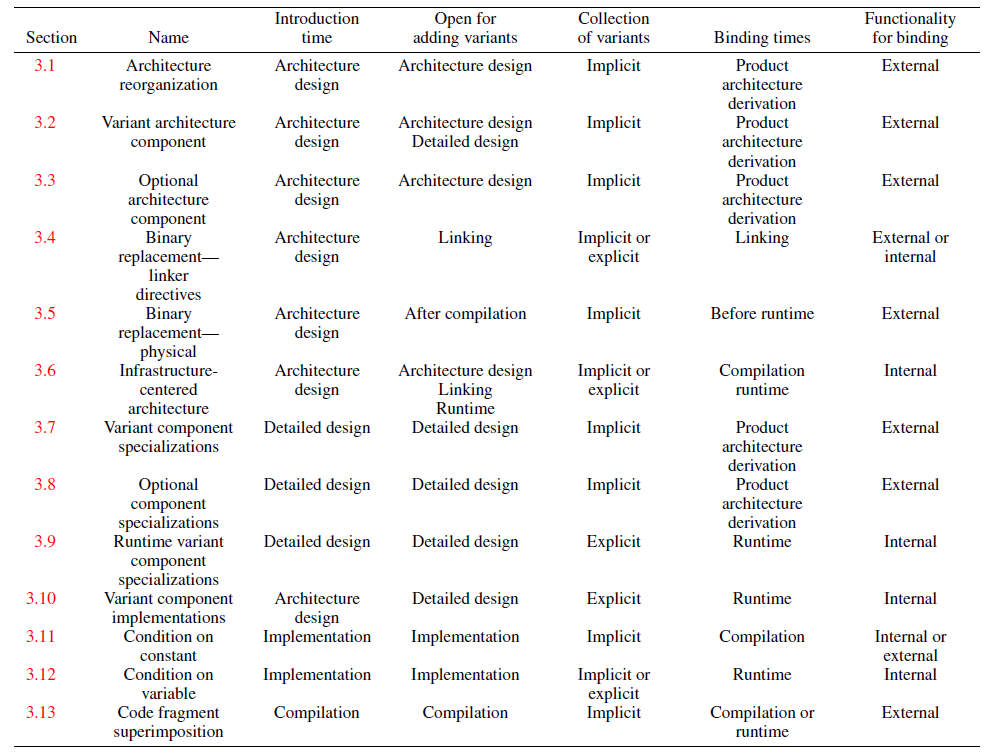
\includegraphics[width=1.0 \textwidth]{figure/figure3.png}
%
%\caption{ Summary of realization mechanisms. Taken from (Svahnberg, van Gurp \& Bosch, 2005 p742)}
%\end{figure*}

We preferred a solution which does not require major architectural restructuring, as this would interfere with the company's current approaches. For this reason, we focused on two techniques, \textit{Variant component} specializations and \textit{Optional component specializations} as they comply with the identified indicators. 
In the next chapter we provide more details about the method we choose to follow and the reasoning behind it. 
